% !TeX spellcheck = en_us

\section{Introduction}
\begin{enumerate}
	
\item  Problem 1: Reasoning about system is hard\\
Source: General / abstract documentation is either:
\begin{enumerate}
	\item far away from the code (e.g., in wikis or other external documents) => hardly maintained, not directly visible to the developer
	\item or scattered through the code (duplication of documentation) => update anomaly, hard to find all comment instances, 
\end{enumerate}

\item  Problem 2: Finding all code instances for a cross-cutting concern is hard\\
Source: scatted code, not pointers to all code instances

\end{enumerate}


Code comment classification\cite{Pascarella2017ClassifyingCodeComments} 
\section{Background}

\subsection{Code Documentation}

\section{Concept}

\begin{itemize}
\item commentary discusses concerns that cross-cut executable dev. artifacts (e.g., methods, classes)
\item pull comments out of the source code 
\item commentary references development artifacts 
\end{itemize}

\section{Related Work}

\section{Discussion}

\section{Conclusion}

\begin{figure}
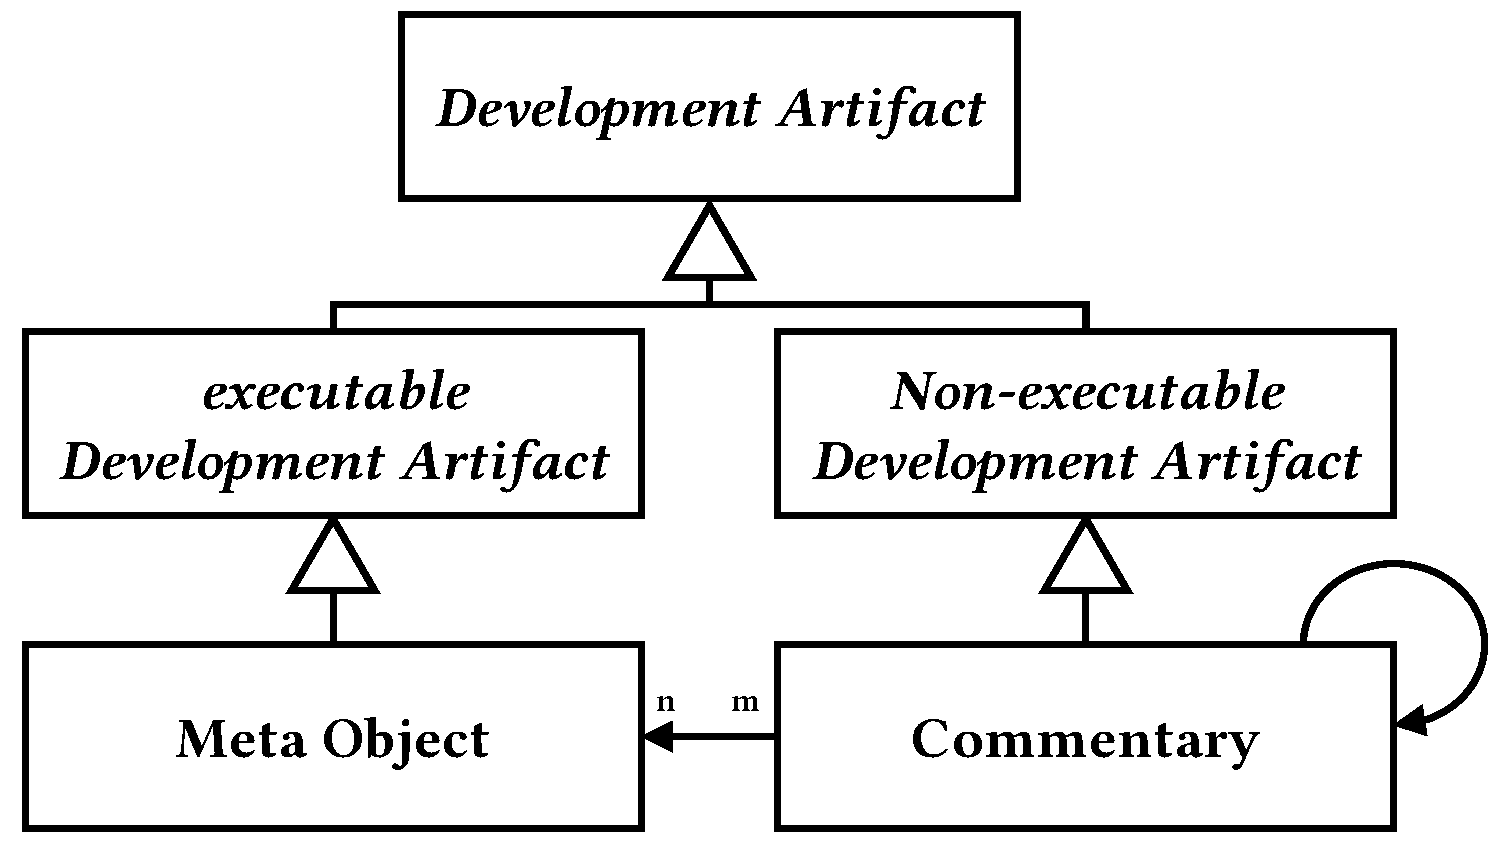
\includegraphics[page=1, width=\columnwidth]{images/metamodel}
\caption{Meta model}
\end{figure}
%\section*{Acknowledgments}